
% ----------------------------------------------------------------------
%  Set the document class
% ----------------------------------------------------------------------
\documentclass[11pt,a4paper,twoside]{article}

% ----------------------------------------------------------------------
% Define external packages, language, margins, fonts and new commands
% ----------------------------------------------------------------------
%\input{preamble} 
\usepackage[utf8]{inputenc}   % <<<<< Linux
\usepackage[english]{babel} % <<<<< English
\usepackage{notoccite}
\usepackage[skip=0.5\baselineskip]{caption}
\hyphenation{GTKWave}
\usepackage{listings}
\usepackage[all]{nowidow}
\usepackage{amsmath}

%blind text
\usepackage{lipsum}

\usepackage{graphicx}
\graphicspath{ {./} {../../figlib/} }
\def\FontLn{% 16 pt normal
  \usefont{T1}{phv}{m}{n}\fontsize{16pt}{16pt}\selectfont}
\def\FontLb{% 16 pt bold
  \usefont{T1}{phv}{b}{n}\fontsize{16pt}{16pt}\selectfont}
\def\FontMn{% 14 pt normal
  \usefont{T1}{phv}{m}{n}\fontsize{14pt}{14pt}\selectfont}
\def\FontMb{% 14 pt bold
  \usefont{T1}{phv}{b}{n}\fontsize{14pt}{14pt}\selectfont}
\def\FontSn{% 12 pt normal
  \usefont{T1}{phv}{m}{n}\fontsize{12pt}{12pt}\selectfont}

% Use Arial font as default
%
\renewcommand{\rmdefault}{phv}
\renewcommand{\sfdefault}{phv}
\usepackage{geometry}	
\geometry{verbose,tmargin=2.5cm,bmargin=2.5cm,lmargin=2.5cm,rmargin=2.5cm}

%\usepackage{setspace}
%\renewcommand{\baselinestretch}{1.5}

\usepackage[pdftex]{hyperref} % enhance documents that are to be
                              % output as HTML and PDF
\hypersetup{colorlinks,       % color text of links and anchors,
                              % eliminates borders around links
%            linkcolor=red,    % color for normal internal links
            linkcolor=black,  % color for normal internal links
            anchorcolor=black,% color for anchor text
%            citecolor=green,  % color for bibliographical citations
            citecolor=black,  % color for bibliographical citations
%            filecolor=magenta,% color for URLs which open local files
            filecolor=black,  % color for URLs which open local files
%            menucolor=red,    % color for Acrobat menu items
            menucolor=black,  % color for Acrobat menu items
%            pagecolor=red,    % color for links to other pages
            pagecolor=black,  % color for links to other pages
%            urlcolor=cyan,    % color for linked URLs
            urlcolor=black,   % color for linked URLs
	          bookmarks=true,         % create PDF bookmarks
	          bookmarksopen=false,    % don't expand bookmarks
	          bookmarksnumbered=true, % number bookmarks
	          pdftitle={report},
            pdfauthor={Andre C. Marta},
%            pdfsubject={Thesis Title},
%            pdfkeywords={Thesis Keywords},
            pdfstartview=FitV,
            pdfdisplaydoctitle=true}

\usepackage[numbers,sort&compress]{natbib} % <<<<< References in numbered list [1],[2],...
\usepackage{subcaption} 
\usepackage{mdframed}
\usepackage{float}

%%%%%%%%%%%%%%%%%%%%%%%%%%%%%%%%%%%%%%%%%%%%%%%%%%%%%%%%%%%%%%%%%%%%%%%%
%     Begin Document                                                   %
%%%%%%%%%%%%%%%%%%%%%%%%%%%%%%%%%%%%%%%%%%%%%%%%%%%%%%%%%%%%%%%%%%%%%%%%


\begin{document}

% Set plain page style (no headers, footer with centered page number)
\pagestyle{plain}

% Set roman numbering (i,ii,...) before the start of chapters
%\pagenumbering{roman}

% ----------------------------------------------------------------------
%  Cover page
% ----------------------------------------------------------------------
%%%%%%%%%%%%%%%%%%%%%%%%%%%%%%%%%%%%%%%%%%%%%%%%%%%%%%%%%%%%%%%%%%%%%%%%
%                                                                      %
%     File: Thesis_FrontCover.tex                                      %
%     Tex Master: Thesis.tex                                           %
%                                                                      %
%     Author: Andre C. Marta                                           %
%     Last modified :  2 Jul 2015                                      %
%                                                                      %
%%%%%%%%%%%%%%%%%%%%%%%%%%%%%%%%%%%%%%%%%%%%%%%%%%%%%%%%%%%%%%%%%%%%%%%%

\thispagestyle {empty}

% IST Logo - Signature A
% parameters: bb=llx lly urx ury (bounding box), width=h_length, height=v_length, angle=angle, scale=factor, clip=true/false, draft=true/false. 
\includegraphics[bb=9.5cm 11cm 0cm 0cm,scale=0.29]{IST_A_CMYK_POS}

\begin{center}
%
% Figure (Image or plot)
\vspace{1.0cm}
% height = 50 mm
%\includegraphics[height=50mm]{Figures/Airbus_A350.jpg}

% Title, author and degree
\vspace{1cm}
{\FontLb Circuit Theory and Electronics Fundamentals} \\ % <<<<< EDIT TITLE
\vspace{1cm}
{\FontSn Department of Electrical and Computer Engineering, Técnico, University of Lisbon} \\ % <<<<< EDIT COURSE
\vspace{1cm}
{\FontSn 5º Laboratory Report} \\
\vspace{1cm}
{\FontSn June 8, 2021} \\ % <<<<< EDIT DATE (corresponds to date of oral examination)
%
\end{center}



% ----------------------------------------------------------------------
% Dedication page (optional)
% ----------------------------------------------------------------------
%\input{dedication} 
%\cleardoublepage

% ----------------------------------------------------------------------
%  Acknowledgments (optional)
% ----------------------------------------------------------------------
%\input{acknowledgements}
%\cleardoublepage

% ----------------------------------------------------------------------
%  Abstract (both in English and Portuguese)
% ----------------------------------------------------------------------
%\input{resumo} 
%\cleardoublepage

%\input{abstract} 

% ----------------------------------------------------------------------
%  Table of contents, list of tables, list of figures and nomenclature
% ----------------------------------------------------------------------

% Table of contents
%
\tableofcontents

% List of tables
%\addcontentsline{toc}{section}{\listtablename}
%\listoftables
%\cleardoublepage 

% List of figures
%\addcontentsline{toc}{section}{\listfigurename}
%\listoffigures
%\cleardoublepage 

% Set arabic numbering (1,2,...) after preface
%
%\setcounter{page}{1}
%\pagenumbering{arabic}

% ----------------------------------------------------------------------
%  Body
% ----------------------------------------------------------------------

\section{Introduction}
\label{sec:introduction}



% state the learning objective 
The objective of this laboratory assignment is to dimension and implement a BandPass Filter (BPF) with a central frequency of 1kHz and a gain at central frequency of 40dB. 
In order to build the circuit, we used 4 resistors, 2 capacitors and a 741 OPAMP.
 

In section 2, a theoretical analysis of the circuit is presented. In section 3, the circuit's simulation analysis results are expressed in graphics and commented. Finally, in section 4, we will compare the simulation and theoretical values and in this way conclude our study.




\section{Theoretical Analysis}
\label{sec:analysis}

In the following subsections, we will explain the theoretical analysis made to predict the output voltages and impedance in the Gain and Output, designed by the teacher previously.
It's important to mention that the gain stage and output parameters are in the same table and the gain stage and output stage results as well.

\subsection{Gain Stage}

In the table below we have the most important values used to design the circuit for the gain stage:
\begin{table}[H]
	\centering
	\begin{tabular}{|l|r|}
		\hline    
		{\bf Name} & {\bf Value [mA]} \\ \hline
		VT & 0.025000 \\  \hline 
BFN & 178.700000 \\  \hline 
VAFN & 69.700000 \\  \hline 
RE1 & 0.100000 K\\  \hline 
RC1 & 1.000000 K\\  \hline 
RB1 & 80.000000 K\\  \hline 
RB2 & 20.000000 K\\  \hline 
VBEON & 0.700000 \\  \hline 
VCC & 12.000000 \\  \hline 
RS & 0.100000 K\\  \hline 
BFP & 227.300000 K\\  \hline 
VAFP & 37.200000 \\  \hline 
RE2 & 0.100000 K\\  \hline 
VEBON & 0.700000 \\  \hline 
C I & 1000.000000 u\\  \hline 
C E & 1000.000000 u\\  \hline 
C O & 1.000000 u\\  \hline 

	\end{tabular}
	\caption{Octave Parameters}
	\label{tab:op}
\end{table}

The circuit is constituted by tow stages, an initial stage with an high input and output impedance, and a second stage a high input impedance, low output impedance and with a gain close to one.
The results we obtained, by the method described above, are present in the following table
\begin{table}[H]
	\centering
	\begin{tabular}{|l|r|}
		\hline    
		{\bf Name} & {\bf Value [mA]} \\ \hline
		V eq & 2.400000 K\\  \hline 
I B & 0.050044 m\\  \hline 
I c 1 & 8.942891 m\\  \hline 
I e 1 & 8.992935 m\\  \hline 
V E & 0.899293 \\  \hline 
V Output 1 & 3.057109 \\  \hline 
VCE & 2.157816 \\  \hline 
V Input 2 & 3.057109 \\  \hline 
I c 2 & 82.067853 m\\  \hline 
I e 2 & 82.428908 m\\  \hline 
V Output & 3.757109 \\  \hline 

	\end{tabular}
	\caption{Octave operating point results}
	\label{tab:op}
\end{table}
	
If we pay attention to the values obtained, we notice that the output impedance is too high, so the circuit cannot be connected to an 80hm load and, therefore, we need an output stage.
\subsection{Output Stage}
As mentioned previously, we need the output stage to induce a low impedance to the load and the parameters for this circuit are shown below:

\begin{table}[H]
	\centering
	\begin{tabular}{|l|r|}
		\hline    
		{\bf Name} & {\bf Value [mA]} \\ \hline
		VT & 0.025000 \\  \hline 
BFN & 178.700000 \\  \hline 
VAFN & 69.700000 \\  \hline 
RE1 & 0.100000 K\\  \hline 
RC1 & 1.000000 K\\  \hline 
RB1 & 80.000000 K\\  \hline 
RB2 & 20.000000 K\\  \hline 
VBEON & 0.700000 \\  \hline 
VCC & 12.000000 \\  \hline 
RS & 0.100000 K\\  \hline 
BFP & 227.300000 K\\  \hline 
VAFP & 37.200000 \\  \hline 
RE2 & 0.100000 K\\  \hline 
VEBON & 0.700000 \\  \hline 
C I & 1000.000000 u\\  \hline 
C E & 1000.000000 u\\  \hline 
C O & 1.000000 u\\  \hline 

	\end{tabular}
	\caption{Octave parameters}
	\label{tab:op}
\end{table}


As seen before, the operating point and incremental analysis were acquired in order to find the output impedance and gain.
The results can be seen below: 
\begin{table}[H]
	\centering
	\begin{tabular}{|l|r|}
		\hline    
		{\bf Name} & {\bf Value [mA]} \\ \hline
		V eq & 2.400000 K\\  \hline 
I B & 0.050044 m\\  \hline 
I c 1 & 8.942891 m\\  \hline 
I e 1 & 8.992935 m\\  \hline 
V E & 0.899293 \\  \hline 
V Output 1 & 3.057109 \\  \hline 
VCE & 2.157816 \\  \hline 
V Input 2 & 3.057109 \\  \hline 
I c 2 & 82.067853 m\\  \hline 
I e 2 & 82.428908 m\\  \hline 
V Output & 3.757109 \\  \hline 

	\end{tabular}
	\caption{Octave operating point results}
	\label{tab:op}
\end{table}

Our objective was to get a gain for the output stage as close to one as possible and a low output impedance, which is exactly what we accomplished and it also means that its ideal to connect the load.

\subsection{Total Results}
Lastly, we will analyze the frequency response of the gain and plot it into a graphic as the one below. 

The graphics of the voltage deviation is:
\begin{figure}[H] \centering
\includegraphics[width=0.6\linewidth]{magnitude_response_gain.eps}
\caption{Voltage deviation plot}
\label{fig:rc4}
\end{figure}

The results (of higher importance) obtained for the total circuit are shown in the next table: 

\begin{table}[H]
	\centering
	\begin{tabular}{|l|r|}
		\hline    
		{\bf Name} & {\bf Value [mA]} \\ \hline
		V eq & 2.400000 K\\  \hline 
I B & 0.050044 m\\  \hline 
I c 1 & 8.942891 m\\  \hline 
I e 1 & 8.992935 m\\  \hline 
V E & 0.899293 \\  \hline 
V Output 1 & 3.057109 \\  \hline 
VCE & 2.157816 \\  \hline 
V Input 2 & 3.057109 \\  \hline 
I c 2 & 82.067853 m\\  \hline 
I e 2 & 82.428908 m\\  \hline 
V Output & 3.757109 \\  \hline 

	\end{tabular}
	\caption{Total circuit results}
	\label{tab:op}
\end{table}

Just by observing this results, we can understand that both stages can be connected without any major signal loss and the reason is that the output impedance is significantly smaller than the input impedance of the output stage.

\section{Simulation Analysis}
\label{sec:simulation}

\subsection{Operating point Analysis (for t<0 and Vs(t) = 0)}

Ngspice was used to perform an operating point analysis for t<0 (obtaining the table below) and by setting $v_s = 0$ and replacing the capacitor with a voltage sorce $V_x = V_6 - V_8$, the voltage and current values, present in tables below, were obtained.

\begin{table}[H]
	\centering
	\begin{tabular}{|l|r|}
		\hline    
		{\bf Name} & {\bf Value [mA]} \\ \hline
		@c[i] & 0.000000e+00\\ \hline
@g1[i] & -2.54235e-04\\ \hline
@r1[i] & 2.428134e-04\\ \hline
@r2[i] & -2.54235e-04\\ \hline
@r3[i] & -1.14215e-05\\ \hline
@r4[i] & 1.174094e-03\\ \hline
@r5[i] & -2.54235e-04\\ \hline
@r6[i] & 9.312805e-04\\ \hline
@r7[i] & 9.312805e-04\\ \hline
v(1) & 5.026261e+00\\ \hline
v(2) & 4.779742e+00\\ \hline
v(3) & 4.248216e+00\\ \hline
v(4) & 4.815245e+00\\ \hline
v(5) & 5.586461e+00\\ \hline
v(6) & -1.87151e+00\\ \hline
v(7) & -2.80798e+00\\ \hline
v(8) & -1.87151e+00\\ \hline

	\end{tabular}
	\caption{Current and voltage results obtained with Ngspice for t<0 }
	\label{tab:op}
\end{table}



\begin{table}[H]
	\centering
	\begin{tabular}{|l|r|}
		\hline    
		{\bf Name} & {\bf Value [mA]} \\ \hline
		@c[i] & 0.000000e+00\\ \hline
@g1[i] & -2.54235e-04\\ \hline
@r1[i] & 2.428134e-04\\ \hline
@r2[i] & -2.54235e-04\\ \hline
@r3[i] & -1.14215e-05\\ \hline
@r4[i] & 1.174094e-03\\ \hline
@r5[i] & -2.54235e-04\\ \hline
@r6[i] & 9.312805e-04\\ \hline
@r7[i] & 9.312805e-04\\ \hline
v(1) & 5.026261e+00\\ \hline
v(2) & 4.779742e+00\\ \hline
v(3) & 4.248216e+00\\ \hline
v(4) & 4.815245e+00\\ \hline
v(5) & 5.586461e+00\\ \hline
v(6) & -1.87151e+00\\ \hline
v(7) & -2.80798e+00\\ \hline
v(8) & -1.87151e+00\\ \hline

	\end{tabular}
	\caption{Current and voltage results obtained with Ngspice for Vs = 0}
	\label{tab:op}
\end{table}


\subsection{Transient Analysis - Natural Response}

The first step in order to compute the natural response of $v_6$ is to set $v_s(t) = 0$ and set initial conditions so that $v_6$ and $v_s$ have the same values obtained in table 10, which ensures that in the start of the transient analysis the capacitor is fully charged. The graphic in figure 11 was obtained by executing a transient analysis, with t ranging from o to 20 ms.

By analyzing the graphic we can see a quick drop in voltage from just a little above 8 ms to 0, which is due to the fact that the capacitor is just discharging and since there are no independent voltage sources, there is no voltage being provided to $v_6$.

\begin{figure}[H] \centering
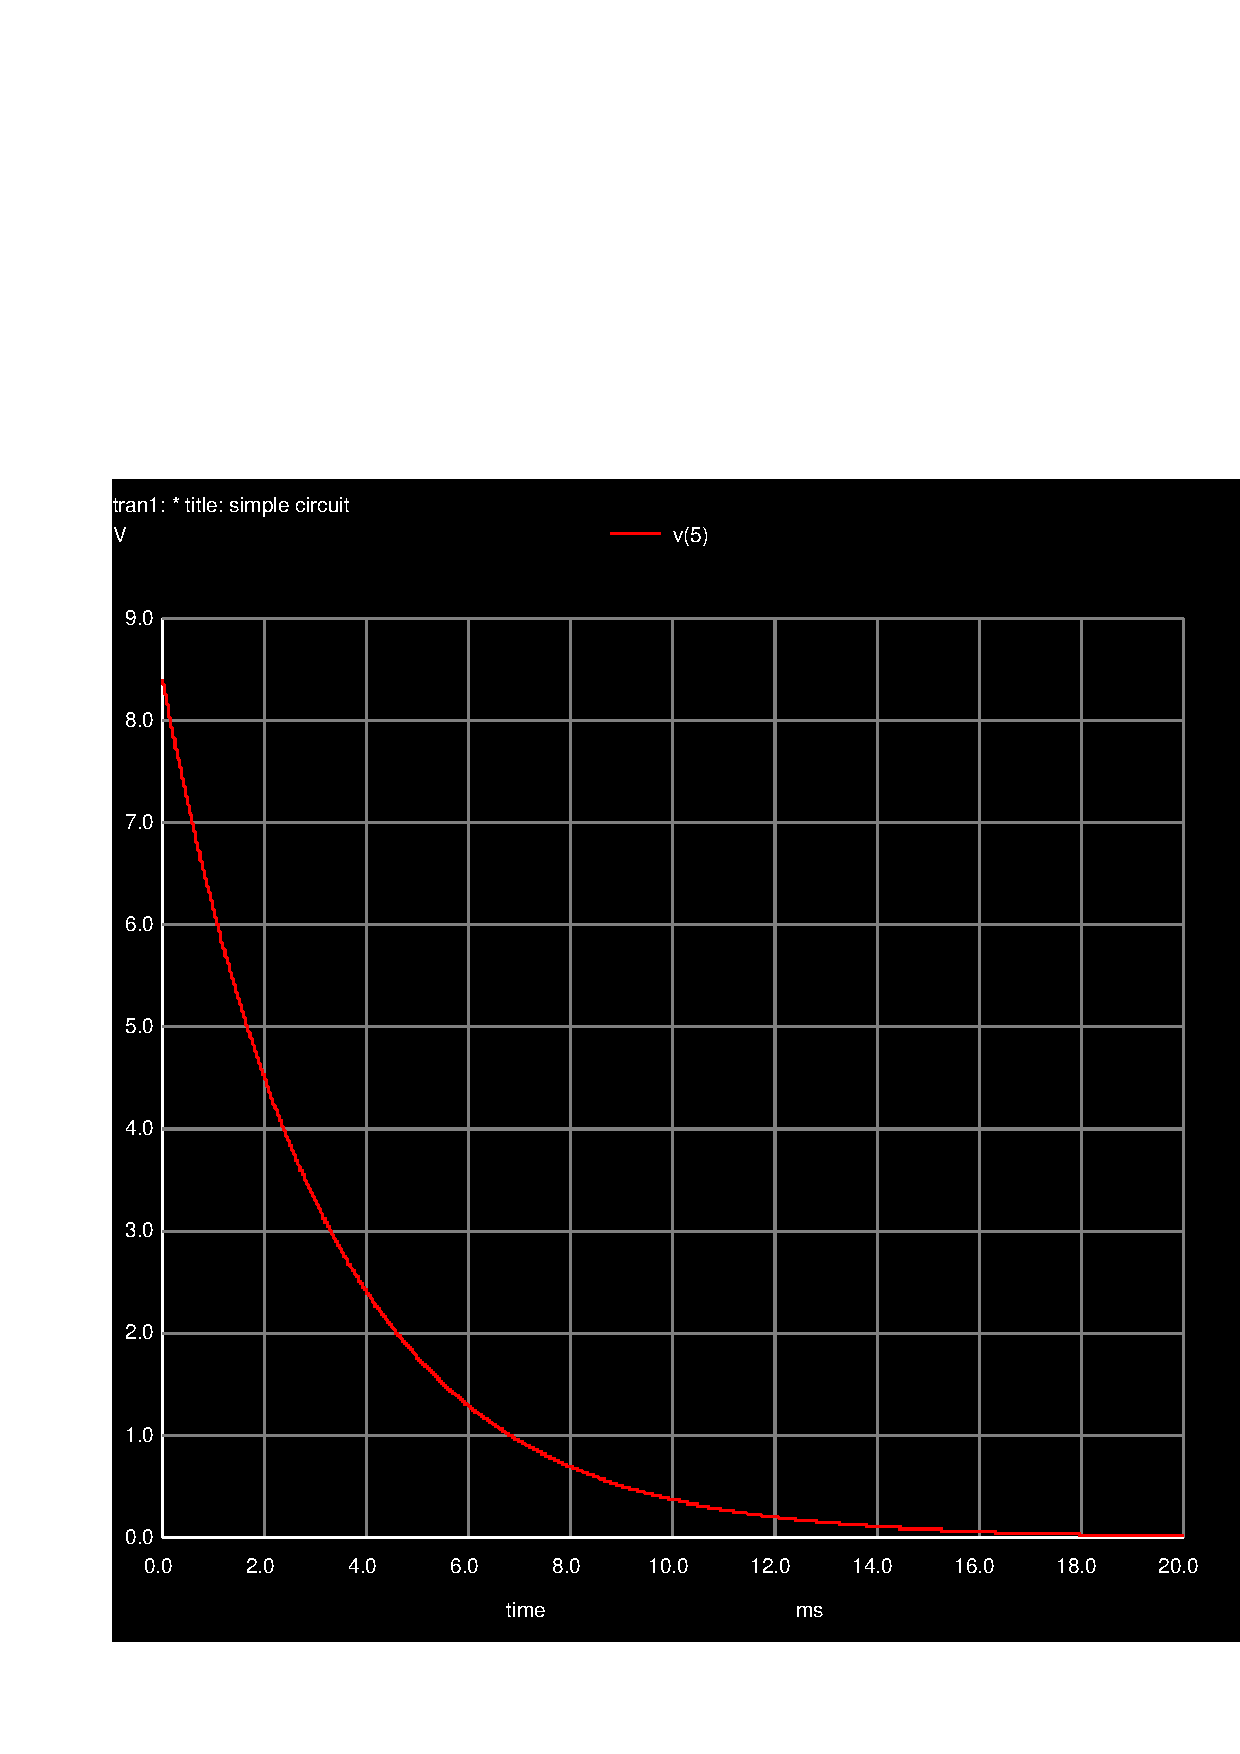
\includegraphics[width=0.6\linewidth]{trans.pdf}
\caption{Natural response}
\label{fig:rc1}
\end{figure}


\subsection{Transient Analysis - total Response}

Taking in consideration that $v_s(t) = \sin(2\pi ft)$ and f = 1000Hz, the total response can be obtained by performing a transient analysis and the figure 12 can be obtained by plotting $v_s(t)$ and $v_6(t)$. 

\begin{figure}[H] \centering
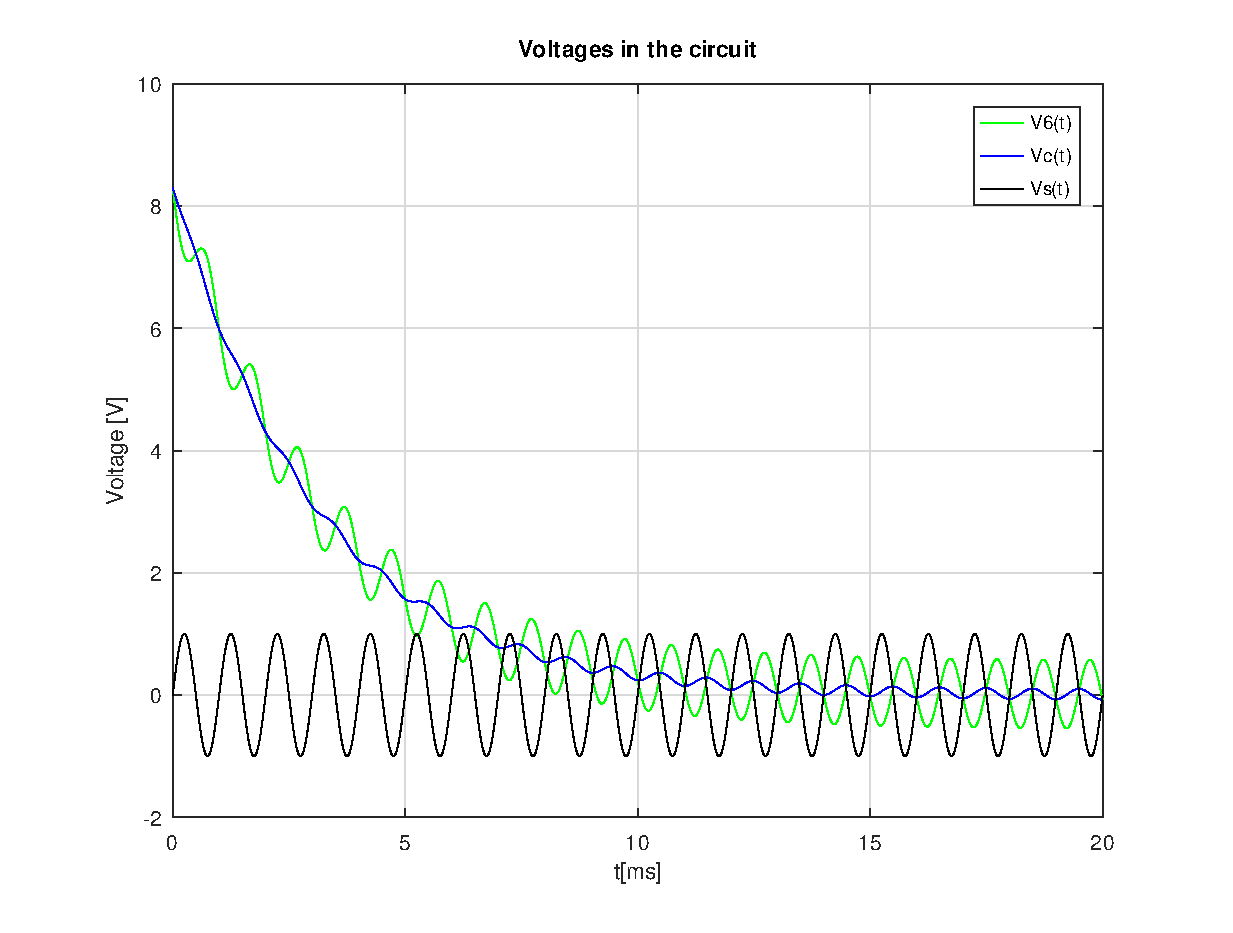
\includegraphics[width=0.6\linewidth]{global_voltage.eps}
\caption{Stinulus voltage ,$v_s(t)$, shown in black and total response, $v_6(t)$, shown in green}
\label{fig:rc1}
\end{figure}


\subsection{Frequency Response}

By excuting a frequency sweep, throughout the length of the interval [0.1, 1000000], we are able to plot the magnitude and phase, which appear below respectively.
\begin{figure}[H] \centering

\includegraphics[width=0.6\linewidth]{acm.pdf}
\caption{Magnitude plot}
\label{fig:rc1}
\end{figure}



\begin{figure}[H] \centering
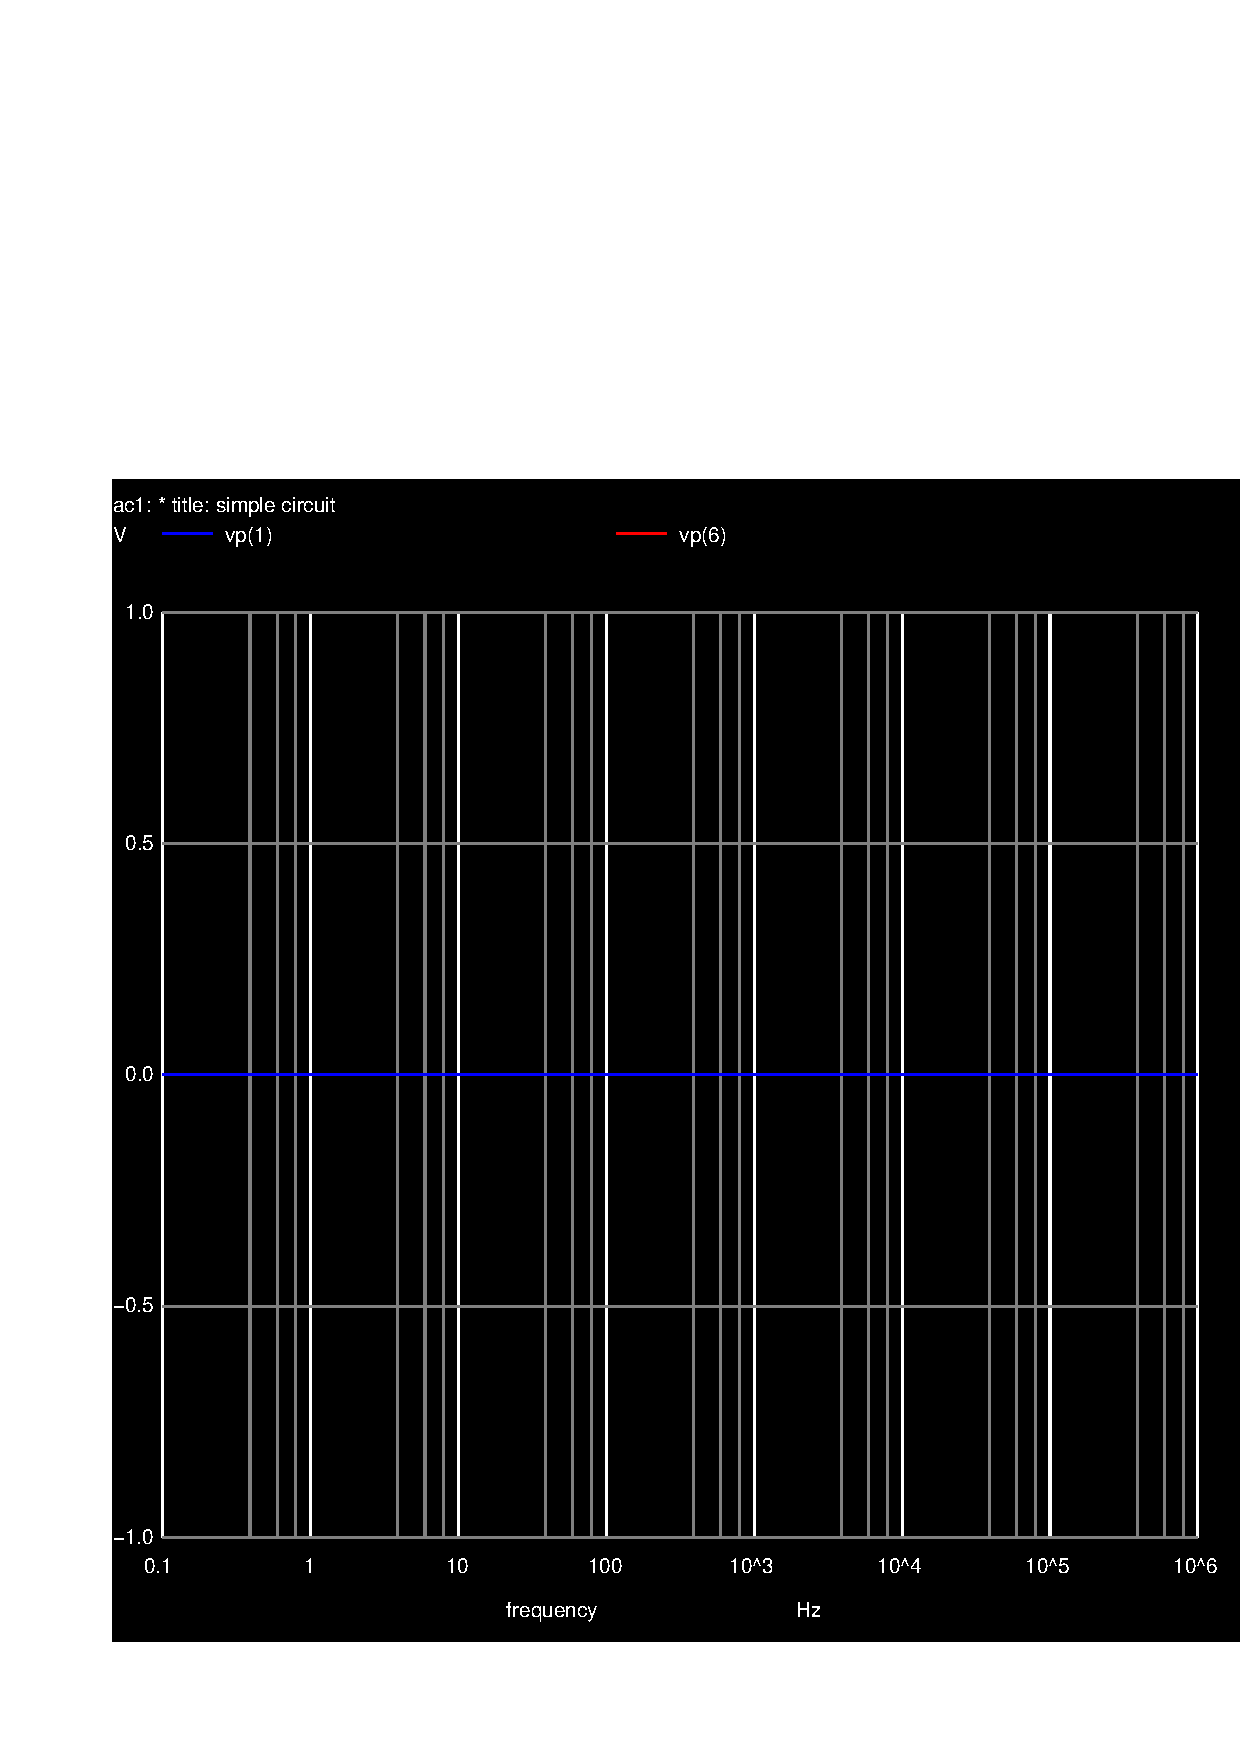
\includegraphics[width=0.6\linewidth]{acp.pdf}
\caption{Phase plot}
\label{fig:rc1}
\end{figure}



\section{Conclusion}
\label{sec:conclusion}
To summarize, the deviation between the theoretical and simulated vales, was higher than what we were expecting, however, this doesn't mean our methods aren't a good aproximation or that they cannot be used to simulate the circuit used in this lab assignment. The errors we obtained are most likely due to some mistakes made when writing the code and the circuit equations in octave and can be fixed.
In conclusion, we should also mention that the cost we obtained for our circuit was slightly higher than we hoped for (the cost was 325,48 monetary units), but it was necessary. 
%\cleardoublepage

% ----------------------------------------------------------------------
%  Bibliography
% ----------------------------------------------------------------------
%\addcontentsline{toc}{section}{\bibname}
%\bibliographystyle{abbrvunsrtnat} % <<<<< SELECT IF USING REFERENCES BY NUMBER (CITATION ORDER)
%\bibliography{../../../BIBfile.bib}

% ----------------------------------------------------------------------
\end{document}
% ----------------------------------------------------------------------

